\chapter{Implementation}
\label{chap:impl}

\Crefname{equation}{Eq.}{Eqs.}
\Crefname{figure}{Fig.}{Figs.}
\Crefname{tabular}{Tab.}{Tabs.}

\texttt{clerk} produces a styled spreadsheet with data and formulas on it. These formulas are evaluated when the document is loaded into a target spreadsheet system.
\Cref{sec:ex3} demonstrates construction of a table for volume and pressure. \Cref{sec:styles} provides the expressions for styling the tables.

\section{Example 3. Volume and pressure}
\label{sec:ex3}

This sections describes the generation of a spreadsheet which calculates the pressure data given some volume data and constants. The program produces an \texttt{xlsx} file that looks as in \Cref{fig:volumePressure}.

\begin{figure}[h]
  \centering
  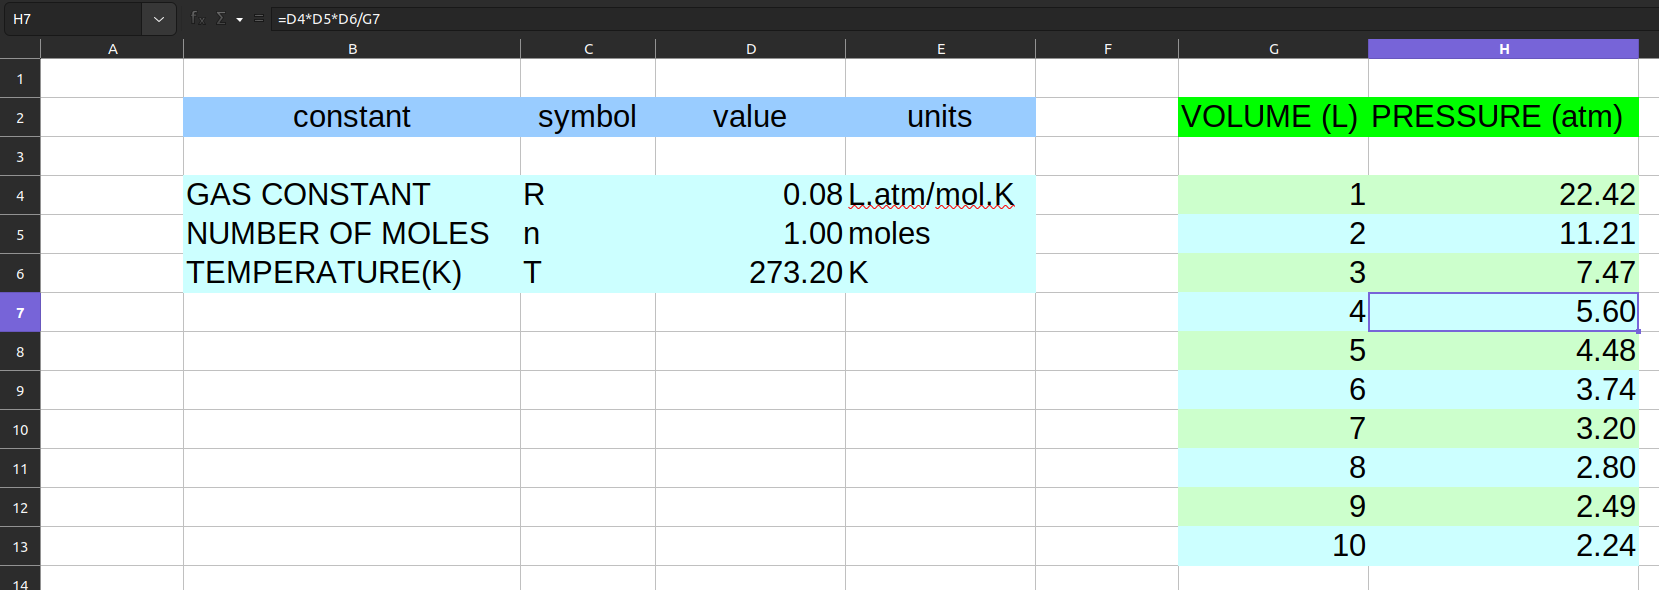
\includegraphics[scale=0.3]{Chapter4/volumePressure.png}
  \caption{Volume and pressure table}
  \label{fig:volumePressure}
\end{figure}

With formulas enabled, I obtained a spreadsheet as in \Cref{fig:volumePressureFormulas}.

\begin{figure}[h]
  \centering
  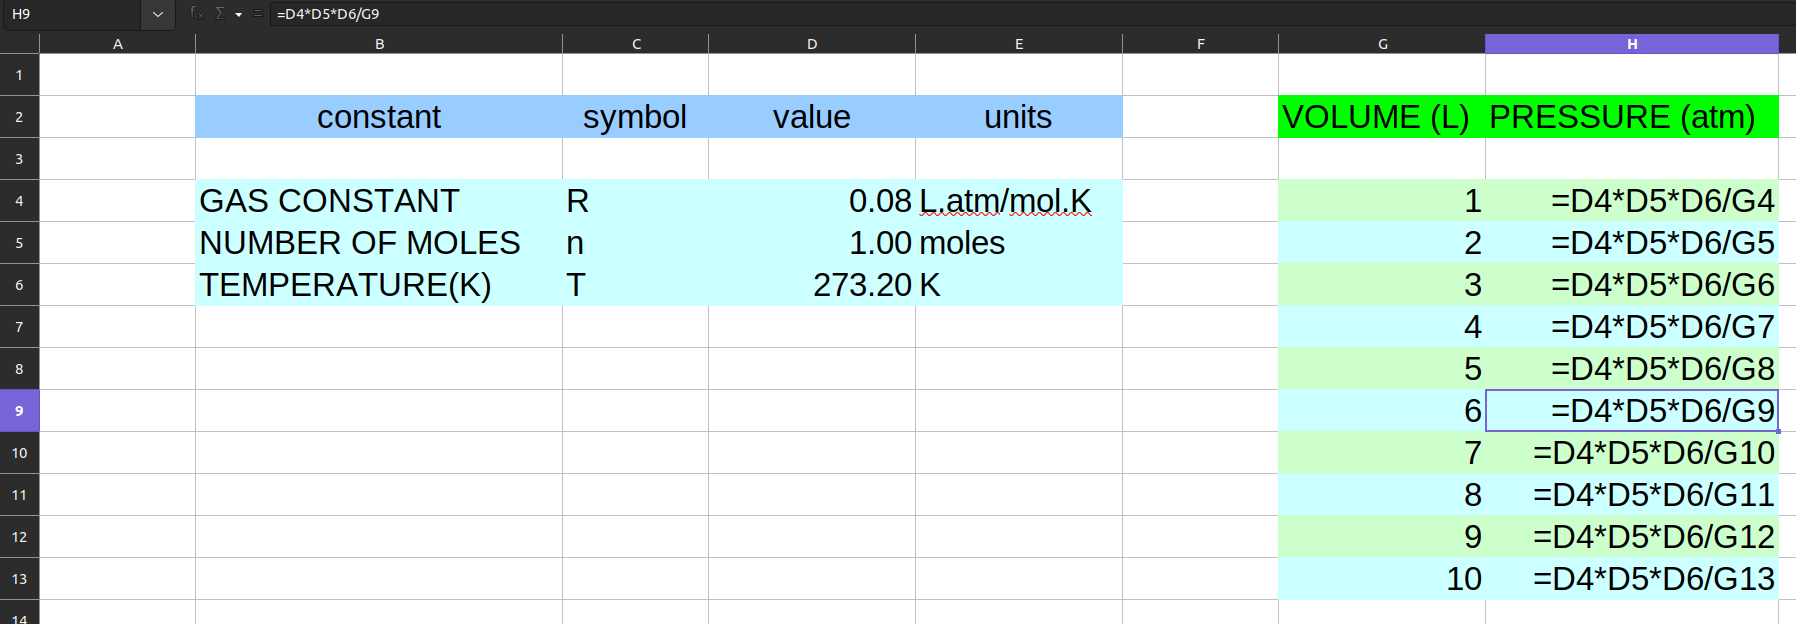
\includegraphics[scale=0.3]{Chapter4/volumePressureFormulas.png}
  \caption{Volume and pressure table with formulas enabled}
  \label{fig:volumePressureFormulas}
\end{figure}

\subsection{Extensions}

I enabled several language extensions so that the compiler could recognize the necessary language features.

% SINGLE_LINE FOURMOLU_DISABLE

\begin{mycode}
{-# LANGUAGE DuplicateRecordFields #-}
{-# LANGUAGE ImportQualifiedPost #-}
{-# LANGUAGE InstanceSigs #-}
{-# LANGUAGE LambdaCase #-}
-- to access the fields of records like a.b
{-# LANGUAGE OverloadedRecordDot #-}
{-# LANGUAGE RankNTypes #-}
{-# LANGUAGE RecordWildCards #-}
{-# LANGUAGE ScopedTypeVariables #-}
\end{mycode}

% SINGLE_LINE FOURMOLU_ENABLE

% LIMA_DISABLE

% module Chapter4_3 where

% LIMA_ENABLE

\subsection{Imports}

Next, I imported the necessary Modules.

\begin{mycode}
import Clerk
import Codec.Xlsx qualified as X
import Codec.Xlsx.Formatted qualified as X
import Data.Text qualified as T
import Lens.Micro ((%~), (&), (+~), (?~))
\end{mycode}

\subsection{Tables}

The tables that I was going to construct were:

- A table per a constant's value (three of them)
- A volume and pressure table
- A constants' header
- A volume and pressure header

\subsubsection{Constants values}

\begin{figure}[h]
  \centering
  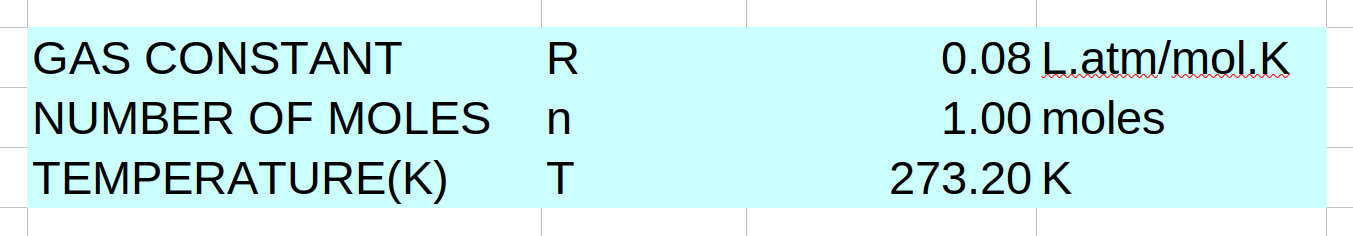
\includegraphics[scale=0.3]{Chapter4/constants.png}
  \caption{Constants values table}
  \label{fig:constants}
\end{figure}

In my case, each constant had the same type of the numeric value - `Double`.
That is why, I constructed a table with a single row per a constant and later placed the constants' tables under each other. I stored constant data in a record.

\begin{mycode}
data ConstantData a = ConstantData
  { constantName :: String
  , constantSymbol :: String
  , constantValue :: a
  , constantUnits :: String
  }
\end{mycode}

Next, I grouped the constants into a record. The parameter \texttt{f} may be an arbitrary type of kind \texttt{* -> *}.

\begin{mycode}
data Constants f = Constants
  { gasConstant :: f Double
  , numberOfMoles :: f Double
  , temperature :: f Double
  }

type ConstantsInput = Constants ConstantData
\end{mycode}

Following that, I recorded the constants data.

\begin{mycode}
constants :: ConstantsInput
constants =
  Constants
    { gasConstant =
        ConstantData "GAS CONSTANT" "R" 0.08206 "L.atm/mol.K"
    , numberOfMoles =
        ConstantData "NUMBER OF MOLES" "n" 1 "moles"
    , temperature =
        ConstantData "TEMPERATURE(K)" "T" 273.2 "K"
    }
\end{mycode}

Now, I made a \texttt{RowI} for a constant input.
I used a \texttt{RowI} because this row requires the input type.
I would later use this row for each constant separately.

I got a pair of outputs:

- Top left cell of a constant table. That is, the cell with that constant name.
- The value of the constant.

Later, I would use these outputs to relate the positions of tables on a sheet.

Here, I used \texttt{lightBlue} from the \Cref{sec:styles}.

\begin{mycode}
constant :: ToCellData a => RowI (ConstantData a) (Ref (), Ref a)
constant = do
  refTopLeft <- columnRef lightBlue constantName
  column lightBlue constantSymbol
  refValue <- columnRef (lightBlue .& with2decimalDigits) constantValue
  column lightBlue constantUnits
  return (refTopLeft, refValue)
\end{mycode}

\subsubsection{Volume and pressure values}

\begin{figure}[h]
  \centering
  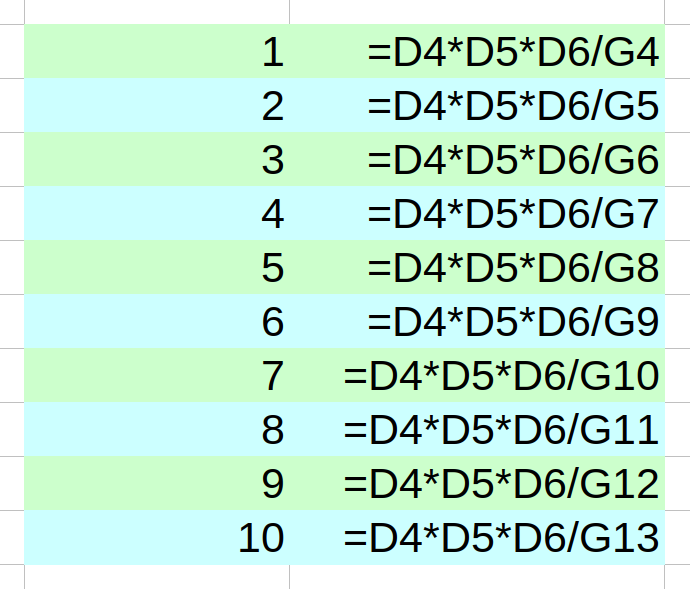
\includegraphics[scale=0.3]{Chapter4/valuesFormulas.png}
  \caption{Volume and pressure table with formulas enabled}
  \label{fig:valuesFormulas}
\end{figure}

I used the data and combined it with the constants to fill table \Cref{fig:valuesFormulas}

\begin{mycode}
newtype Volume = Volume {volume :: Double}

volumeData :: [Volume]
volumeData = Volume <$> [1 .. 10]
\end{mycode}

I made a helper type to pass the constants references in a structured way.

\begin{mycode}
data ConstantsRefs = ConstantsRefs
  { refGasConstant :: Ref Double
  , refNumberOfMoles :: Ref Double
  , refTemperature :: Ref Double
  }
\end{mycode}

Next, I defined a function to produce a row for volume and pressure.

\begin{mycode}
values :: ConstantsRefs -> RowI Volume ()
values ConstantsRefs{..} = do
  refVolume <- columnRef alternatingColors volume
  let pressure' = refGasConstant .* refNumberOfMoles .* refTemperature ./ refVolume
  column (alternatingColors .& with2decimalDigits) (const pressure')
\end{mycode}

\subsubsection{Constants' header}

\begin{figure}[h]
  \centering
  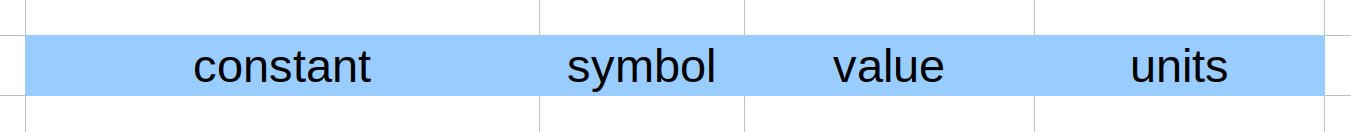
\includegraphics[scale=0.3]{Chapter4/constantsHeader.png}
  \caption{Constants header}
  \label{fig:constantsHeader}
\end{figure}

I did not use records here. Instead, I put the names of the columns straight into the `Row`. The outputs were the coordinates of the top left cell and the top right cell of this table.

\begin{mycode}
constantsHeader :: Row (Ref (), Ref ())
constantsHeader = do
  let style :: FormatCell
      style = blue .& alignedCenter
  refTopLeft <- columnWidthRef 20 style (const "constant")
  columnWidth 8 style (const "symbol")
  column style (const "value")
  refTopRight <- columnWidthRef 13 style (const "units")
  return (refTopLeft, refTopRight)
\end{mycode}

\subsubsection{Volume \& Pressure header}

\begin{figure}[h]
  \centering
  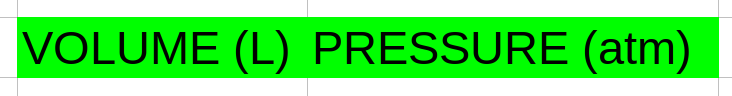
\includegraphics[scale=0.3]{Chapter4/valuesHeader.png}
  \caption{Header for the volume and pressure table}
  \label{fig:valuesHeader}
\end{figure}

For this header, I also put the names of columns straight into a row.

\begin{mycode}
valuesHeader :: Row (Ref ())
valuesHeader = do
  refTopLeft <- columnWidthRef 12 green (const "VOLUME (L)")
  columnWidth 16 green (const "PRESSURE (atm)")
  return refTopLeft
\end{mycode}

\subsection{Sheet builder}

Finally, I combined all rows.

\begin{mycode}
sheet :: Sheet ()
sheet = do
  start <- mkCoords 2 2
  (constantsHeaderTL, constantsHeaderTR) <- place start constantsHeader
  (gasTL, gas) <- place1 (constantsHeaderTL & row +~ 2) constants.gasConstant constant
  (nMolesTL, nMoles) <- place1 (gasTL & row +~ 1) constants.numberOfMoles constant
  temperature <- snd <$> place1 (nMolesTL & row +~ 1) constants.temperature constant
  valuesHeaderTL <- place (constantsHeaderTR & col +~ 2) valuesHeader
  placeN (valuesHeaderTL & row +~ 2) volumeData (values $ ConstantsRefs gas nMoles temperature)
\end{mycode}

\subsection{Styles}
\label{sec:styles}

Below, I list the expressions used for sheet styling.

\begin{mycode}
data Colors = LightBlue | LightGreen | Blue | Green
instance ToARGB Colors where
  toARGB :: Colors -> String
  toARGB = \case
    LightBlue -> "90CCFFFF"
    LightGreen -> "90CCFFCC"
    Blue -> "FF99CCFF"
    Green -> "FF00FF00"

blue :: FormatCell
blue = mkColor Blue

lightBlue :: FormatCell
lightBlue = mkColor LightBlue

green :: FormatCell
green = mkColor Green

alternatingColors :: FormatCell
alternatingColors coords index = mkColor (if even index then LightGreen else LightBlue) coords index
\end{mycode}

Additionally, I composed an \texttt{FCTransform} for the number format.
Such a transform was used to accumulate cell formatting.

\begin{mycode}
with2decimalDigits :: FCTransform
with2decimalDigits fcTransform =
  fcTransform & X.formattedFormat %~ X.formatNumberFormat ?~ X.StdNumberFormat X.Nf2Decimal
\end{mycode}

Finally, I made a transform for centering the cell contents.

\begin{mycode}
alignedCenter :: FCTransform
alignedCenter = horizontalAlignment X.CellHorizontalAlignmentCenter
\end{mycode}
